\section{\sysname Design}
\label{sec:design}

Section~\ref{sec:model} establishes that SD can benefit from expert caching only when $M_{\mathrm{GPU}} \ge M^*$, and identifies two practical barriers that persist above this threshold: cache-hit-path overhead (Observation~1) and transient working-set overflow (Observation~2). This section presents the \sysname design that addresses these two barriers through two corresponding modules, \emph{Unblock} and \emph{Protect}. Figure~\ref{fig:overview} illustrates the overall architecture, and Table~\ref{tab:designmap} summarizes the mapping from analytical findings to system mechanisms. Throughout this section we assume that $M_{\mathrm{GPU}} \ge M^*$, i.e., the per-layer cache holds at least $S \ge \bar{\wsd}$ slots under LRU replacement.

\begin{table}[t]
\caption{Mapping from analysis findings to \sysname mechanisms.}
\label{tab:designmap}
\centering
\small
\begin{tabular}{lll}
\toprule
Finding & Bottleneck & Mechanism \\
\midrule
Obs.~1: Hit-path overhead & $T_{\mathrm{copy}}$ (scratchpad) & Pool-Direct \\
Obs.~1: Hit-path overhead & $T_{\mathrm{sync}}$ (CPU-GPU sync) & TASER \\
Obs.~1: Hit-path overhead & residual $N_{\mathrm{miss}} \cdot t_{\mathrm{miss}}$ & Oracle prefetch \\
Obs.~1: Hit-path overhead & $T_{\mathrm{kernel}}$ & Kernel tuning \\
Obs.~2: Transient overflow & cascade eviction $\Rightarrow$ $\eta\!\downarrow$ & Draft-guided preload \\
\bottomrule
\end{tabular}
\end{table}

\begin{figure*}[t]
\centering
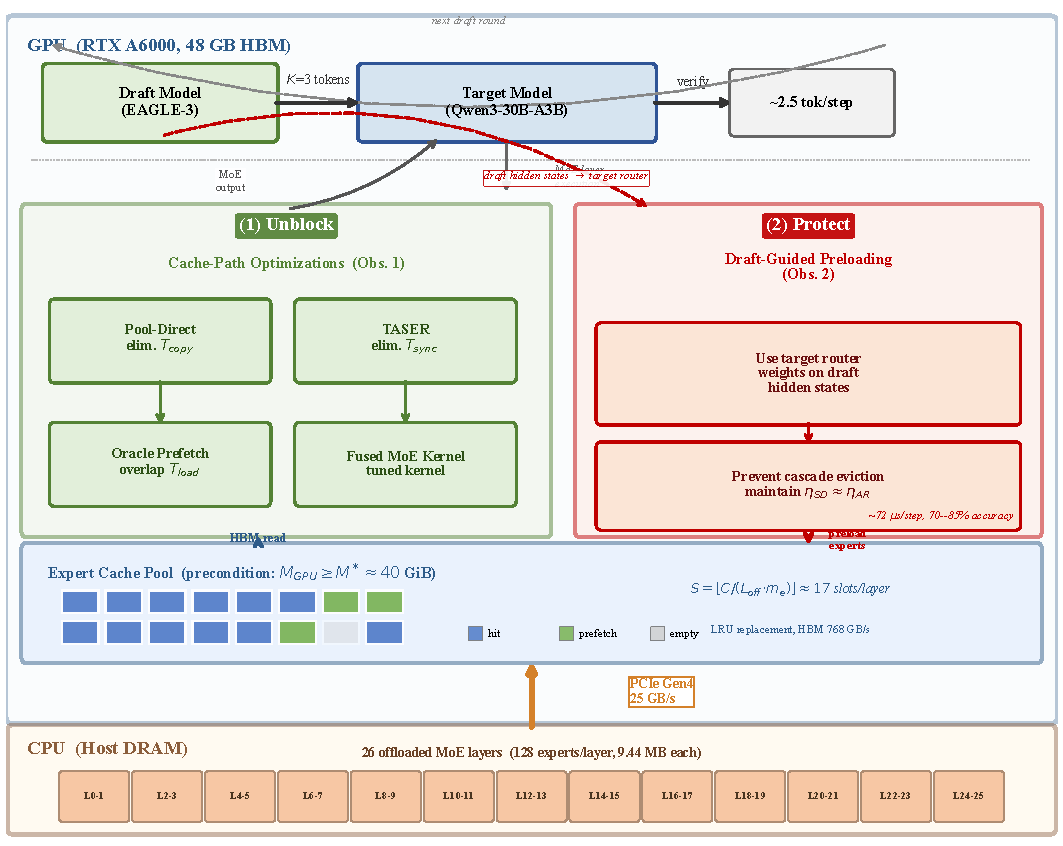
\includegraphics[width=0.95\textwidth]{figures/fig_architecture.pdf}
\caption{\sysname architecture overview. The system operates on top of per-layer expert cache pools (a precondition derived from the $M^*$ threshold in Section~\ref{sec:model}). \emph{Unblock} removes the cache-path bottlenecks identified by Observation~1: Pool-Direct eliminates scratchpad copies ($T_{\mathrm{copy}}$), TASER removes CPU-GPU synchronization ($T_{\mathrm{sync}}$), Oracle Prefetch overlaps residual PCIe transfers ($T_{\mathrm{load}}$), and kernel tuning reduces $T_{\mathrm{kernel}}$. \emph{Protect} addresses Observation~2 by using draft-guided preloading to maintain cache coverage under SD's fluctuating working set.}
\Description{System architecture diagram showing GPU and CPU zones. The GPU zone contains the SD pipeline at top with Draft Model and Target Model, Unblock and Protect optimization modules in the middle, and the CPU zone at bottom contains 26 offloaded MoE layers connected via PCIe.}
\label{fig:overview}
\end{figure*}

\subsection{Unblock: Removing Cache-Path Bottlenecks}

Observation~1 shows that even when the cache covers SD's steady-state working set ($S \ge \bar{\wsd}$), the overhead-to-compute ratio $(T_{\mathrm{copy}} + T_{\mathrm{sync}}) / T_{\mathrm{kernel}} \approx 2.4\times$ limits compute efficiency to 29\%. \sysname removes this overhead through four targeted mechanisms applied in sequence.

\paragraph{Pool-Direct execution.}
A naive cache implementation copies expert weights from the cache pool into a contiguous scratchpad tensor before invoking the fused MoE kernel. This HBM-to-HBM transfer is pure overhead. Pool-Direct eliminates the scratchpad by remapping the kernel's top-$k$ expert IDs into cache-pool slot IDs and executing directly on the pool storage. This design removes $T_{\mathrm{copy}}$ entirely.

\paragraph{TASER.}
After Pool-Direct removes $T_{\mathrm{copy}}$, CPU-GPU synchronization becomes the dominant overhead. Each offloaded layer must perform GPU-to-CPU transfers for \texttt{unique().tolist()}, followed by dictionary lookup, LRU update, and slot remapping on the host. TASER (Temporal-Adaptive Stale Expert Routing) exploits the observation that the expert-to-slot mapping becomes highly stable after warmup: adjacent-step expert overlap exceeds 99\% in steady state (Section~\ref{sec:assumptions}). TASER therefore freezes the mapping and reuses it for most steps, validating it only intermittently via an exponential-backoff schedule. More than 95\% of steps take the fast path, substantially reducing $T_{\mathrm{sync}}$.

\paragraph{Oracle cross-layer prefetch.}
TASER's frozen mapping doubles as a zero-cost oracle for the next layer. When a validation step identifies likely misses in layer $\ell+1$, \sysname prefetches those experts asynchronously while the current layer's kernel executes. This design overlaps residual PCIe transfers with HBM-bound compute, reducing the tail of $N_{\mathrm{miss}} \cdot t_{\mathrm{miss}}$.

\paragraph{Hardware-aware kernel tuning.}
Finally, \sysname tunes the Triton fused-MoE kernel to the A6000 memory hierarchy. The best configuration uses block sizes of 64 and 128 with 8 warps, trimming the remaining $T_{\mathrm{kernel}}$ cost.

\subsection{Protect: Draft-Guided Preloading}

The Unblock module addresses the $\eta$-independent overhead floor but does not prevent the cache-hit rate from degrading under SD's fluctuating working set. As Observation~2 shows, SD's per-step working set ($W_{\mathrm{step}} \approx 19.3$ on average, up to 26.9) frequently exceeds the cache capacity $S \approx 17$, triggering evictions that cascade across ${\sim}8$ subsequent steps (Section~\ref{subsec:obs2}). The Protect module addresses this problem with draft-guided preloading.

During draft generation, the target model is idle. \sysname exploits this window to apply the target router weights to the draft hidden states, predict which experts are likely to be used by the upcoming verification step, and pre-stage those experts into the cache before verification begins. This mechanism is lightweight: the routing prediction costs approximately 72~$\mu$s per step and reaches 70--85\% accuracy. The goal is not aggressive speculative prefetching in general, but specifically maintaining $\eta_{\mathrm{SD}}$ close to $\eta_{\mathrm{AR}}$ by pre-staging the overflow experts before they trigger eviction cascades.

\subsection{Assumptions and Applicability Boundaries}
\label{sec:assumptions}

\sysname inherits the $M^*$ threshold from Section~\ref{sec:model} and introduces additional assumptions through its design choices. We discuss the conditions under which these assumptions hold and the boundaries of applicability.

\paragraph{Cache capacity threshold.}
The effectiveness of \sysname depends on whether $M_{\mathrm{GPU}} \ge M^*$, i.e., the per-layer cache can hold $S \ge \bar{\wsd} \approx 17$ expert slots. With $C = 4$~GB, $L_{\mathrm{off}} = 26$, and $m_e = 9.44$~MB, $S$ is approximately 17. If the available GPU memory shrinks (e.g., due to larger KV caches from longer contexts), $S$ drops below $\bar{\wsd}$ and the per-step overflow worsens: cache misses accumulate across layers and SD provides diminishing returns. Draft-guided preloading partially compensates by maintaining hit rate, but the system operates below its full potential. In the extreme case where $S < \war = 8$, even AR's working set overflows the cache, expert-to-slot mapping churns every step, TASER's fast path is never triggered, and Pool-Direct offers no benefit.

\paragraph{Temporal stability of expert routing.}
TASER and the LRU cache policy both rely on the observation that adjacent decode steps exhibit strong expert routing locality. In our measurements on Qwen3-30B-A3B, adjacent-step expert overlap exceeds 99\% in steady state, and the expert-to-slot mapping stabilizes after approximately 32 warmup steps, reaching $>$99.2\% stability thereafter. MoE architectures with substantially different routing strategies (e.g., hash-based routing~\cite{roller2021hash} or random routing), or input sequences that induce abrupt routing shifts, could reduce the temporal overlap below the threshold needed for TASER's stale mapping to remain valid. Under such conditions, the exponential-backoff schedule would trigger frequent revalidations, diminishing the synchronization savings.

\paragraph{Single-request serving scope.}
\sysname is designed for single-request, batch-size-one, latency-first inference. In this regime, the per-layer working set is bounded by the top-$k$ routing decisions of a single sequence, and expert reuse across nearby steps is high. Batched or concurrent-request serving introduces two complications. First, the union of routing decisions across $B$ requests expands the per-layer working set beyond $\wsd$, potentially pushing $W_{\mathrm{step}}$ permanently above $S$ and triggering persistent overflow even at generous memory budgets. Second, inter-request expert overlap is lower than intra-request overlap, reducing the cache hit rate that TASER's frozen mapping relies on. Large-batch throughput-oriented serving is a qualitatively different problem and is beyond the scope of this work.

\paragraph{Hardware-dependent thresholds.}
The bandwidth ratio $B_{\mathrm{HBM}} / B_{\mathrm{PCIe}} = 30.7$ on our RTX A6000 platform determines the cost disparity between cache hits and misses. On platforms with narrower bandwidth gaps, such as systems using CXL-attached memory or NVLink-connected multi-GPU configurations, the penalty of a cache miss is smaller, which reduces both the absolute benefit of caching and the relative advantage of removing hit-path overhead. Conversely, on platforms with wider gaps (e.g., PCIe Gen3), the benefit is more pronounced. The qualitative structure of the $M^*$ threshold is hardware-independent, but the quantitative values of $M^*$, $t_{\mathrm{miss}}$, and the overhead-to-compute ratio must be recalibrated for each platform.

In summary, \sysname assumes (1) sufficient cache capacity ($M_{\mathrm{GPU}} \ge M^*$), (2) temporally stable expert routing, (3) single-request serving, and (4) a large HBM-to-PCIe bandwidth ratio. When these assumptions hold, the system consistently delivers the improvements demonstrated in Section~\ref{sec:eval}. When they are violated, the system degrades gracefully but does not provide the full speedup reported in this paper.

\subsection{Implementation}

We implement \sysname as a vLLM plugin without modifying the vLLM source tree. The implementation consists of roughly 1{,}500 lines of Python and is controlled through environment variables such as \texttt{VLLM\_PLUGINS=briskmoe} and \texttt{BRISKMOE\_CACHE\_GB=4}. This design keeps the system easy to deploy and makes the cache, stale-routing policy, and preloading logic orthogonal to the rest of the inference stack. Issues concerning multi-GPU sharding and distributed serving are orthogonal to our single-GPU focus and are designated for future work.
